
\chapter{Resonance Search and Results}

The following chapter will discuss the details and results from a resonance 
search conducted on the 2015 engineering run data.  This includes a discussion
of the fit procedure along with the statistical 
formalism used to set a limit.  The chapter will conclude with a discussion 
of systematics.

\section{Searching for a Resonance}

If a heavy photon does indeed exist and has a mass that is within the acceptance
of the HPS detector, it will appear as a resonance above the copious QED trident
invariant mass distribution.  Since the $A'$ signal is unknown a priori, the 
$e^+e^-$ invariant mass is scanned for any significant peaks at a given mass 
hypothesis.  With this in mind, the invariant mass distribution measured by
HPS (see section 4 and Fig. \ref{fig:mass_distribution}) will serve as the 
starting point for this analyses.
\begin{figure}[t]
    \centering
    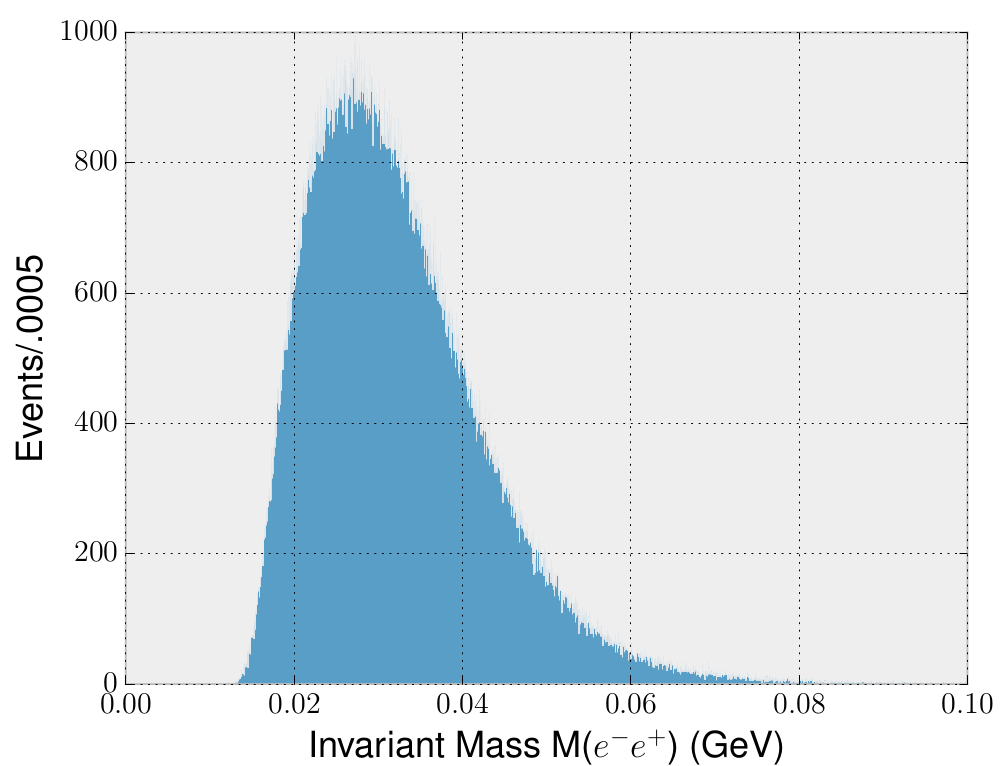
\includegraphics[width=1.0\textwidth]{images/invariant_mass_final.png}
    \caption{The Heavy Photon Search $e^+e^-$ invariant mass distribution after
             the final event selection has been applied.  The mass distribution
             will serve as the starting point for the resonance search.}
    \label{fig:mass_distribution}
\end{figure}

\subsection{Maximum Likelihood Fit}

Customarily, a search for a resonance is perfomed by constructing a
window centered at the mass hypothesis of interest.  Within the window, $A'$ 
signal events are expected to appear as a Gaussian resonance, $\phi$, centered at
the mass hypothesis, $m_{A'}$ and with a width, $\sigma_{m_{A'}}$, equal to the
 measured mass resolution of
the experiment.  The distribution of background events within the same window
can be modeled by a polynomial, $p$ with coefficients $t_j$.  Estimating the 
signal yield, $\mu$, within
the window, as well the background normalization, $B_{total}$ and shape, can be
done by the method of maximum likelihood.  The theoretical formalism
used to do this will be outlined here but a detailed discussion can be found in
\cite{Cowan:2010js}.

Assume the events within the window are binned as $n = (n_{1}, ... n_{i})$.
Furthermore, assume say the center of a bin if given by $b_i$ and has a width
equal to $\epsilon$. 
The expectation value of the $i$th bin in the range is given by 
\begin{equation}
    E[n_i] = S_{i} + B_{i}
\end{equation}
where 
\begin{equation}
    S_{i} = \mu \int_{b_i - \epsilon/2}^{b_i + \epsilon/2} \phi(m_{e^+e^-} | m_{A'}, \sigma_{m_{A'}}) d (m_{e^+e^-})
\end{equation} 
\begin{equation}
    B_{i} = B_{total} \int_{b_i - \epsilon/2}^{b_i + \epsilon/2} poly(m_{e^+e^-} | t_{j}) d (m_{e^+e^-})
\end{equation}
Denoting the nuissance parameters as $\theta = (B_{total},  t_{j})$, and estimation
of $\mu$ and $\theta$ can be obtained by finding the parameters $\hat{\mu}$ and
$\hat{\theta}$ which maximize the Poisson likelihood function $\mathcal{L}$
\begin{equation}
    \mathcal{L}(\mu, \theta) = \prod_{k=1}^{i} \frac{(S_{k} + B_{k})^{n_k}}{n_{k}!} e^{-(S_{k} + B_{k})}. 
\end{equation}
In the case where the invariant mass is scanned for a resonance, the poisson 
likelihood function is maximized and used to estimate the signal yield using a
range of $A'$ mass hypotheses. 

\subsection{Likelihood Ratio}

When searching for a resonance above a distribution of background, it is 
necessary to descriminate between two scenarios:
\begin{itemize}
    \item The background only or null hypothesis, $H_{0}: \mu = 0$.
    \item The signal+background hypothesis or alternative, $H_{1}: \mu > 0$.
\end{itemize}
Establishing whether the signal+background model is significantly different 
from the background only model is typically done using the profile likelihood
ratio
\begin{equation}
    \lambda(0) = \frac{\mathcal{L}(0, \hat{\hat{\theta}})}{\mathcal{L}(\hat{\mu}, \hat{\theta})}
    \label{eqn:likelihood_ratio}
\end{equation}
where $\hat{\hat{\theta}}$ is the conditional estimator for the background 
parameters obtained by maximizing the Poisson likelihood with the assumption
of no signal i.e. background only.  As can be seen from \ref{eqn:likelihood_ratio}, 
if the estimator of the signal yield, $\hat{mu}$ is compatible (incompatible) with the background
only hypothesis i.e. $\mu = 0$, the likelihood ratio will tend to 1 (0).

A more convinient test stastistic is the log likelihood ratio defined as
\begin{equation}
    q_0 = \begin{cases}
            -2 \ln \frac{\mathcal{L}(0, \hat{\hat{\theta}})}{\mathcal{L}(\hat{\mu}, \hat{\theta})} 
            & \hat{\mu} > 0 \\
             0  & \hat{\mu} < 0
        \end{cases}
\end{equation}
According to Wilk's theorem \cite{Wilks:1938dza}, in the large sample limit, the test statistic
$q_0$ is asymptotically $\chi^2$ distributed with degrees of freedom equal to the
difference in parameters between the two models being tested.  In our current case, 
the number of degrees of freedom is one, since the signal yield does not appear in
the background only model.

Quantifying how extreme the observation is, a p-value can be calculated as
\begin{equation}
    p = \int_{q_{0,obs}}^{\infty} f(q_{0} | 0) dq_{0}
\end{equation} 

\subsection{The Look-Elsewhere Effect}

As discussed in previous section, a result is determined signficant if the 
$p$-value is smaller than some pre-determined threshold, $\alpha$.  However, 
when performing multiple test, as is the case when scanning a mass distribution
for a resonance, a observation with a $p$-value that is as extreme as $\alpha$
is bound to occur.  This phenomena is known as the ``Look-Elsewhere Effect'' (LEE)
and needs to be taken into account through a correction to the observed $p$-value
at each mass hypothesis.

Assuming that only a single heavy photon can be observed within the HPS invariant
mass distribution, the correction can be estimated using the distribution 
$f(q_{0, max} | 0)$ composed of the largest $q_{0}$ (i.e. smallest $p$-value)
from each of the invariant mass scans.  The distribution $f(q_{0, max} | 0)$ can
be derived by running a large number of pseudo-experiments and then calculating
the $p$-value as was explained previously.  However, obtaining a ``global''
$p$-value with any accuracy would require running $\sim 10^{6}$ pseudo experiments
which is not feasible.  

Instead, the smallest $p$-values obtained from a modest number of pseudo-experiments were
ranked and the corresponding quantile was calculated.  A mapping from a local 
p-value to a global p-value is then created.  Such a mapping is was created using
10,000 toys and is shown on Fig. \ref{}.  As can be seen from the figure, a 
local p-value equal to 0.05 corresponds to a global p-value of $\sim$ 0.5.

%\section{Optimization of Fit Procedure}

%\subsection{Pseudo Data Sets}

%Pseudo data sets are needed to understand fitting systematics and to optimize
%both
%the fit function and window size.  In order to obtain an invariant mass probability
%density function (PDF) that describes the data, smoothing algorithm 353 QH 
%\cite{Friedman:1974vj} was
% What smoothing algorithm was used? Why? Was a K-S test used to make sure the
% resulting PDF matched the data set?
%applied the unit normalized final invariant mass MC distribution.  The resulting
%PDF after smoothing (blue line) overlayed over the MC distribution it was generated 
%from is shown on Fig. \ref{fig:smooth_pdf}.
%\begin{figure}[b]
%    \centering
%    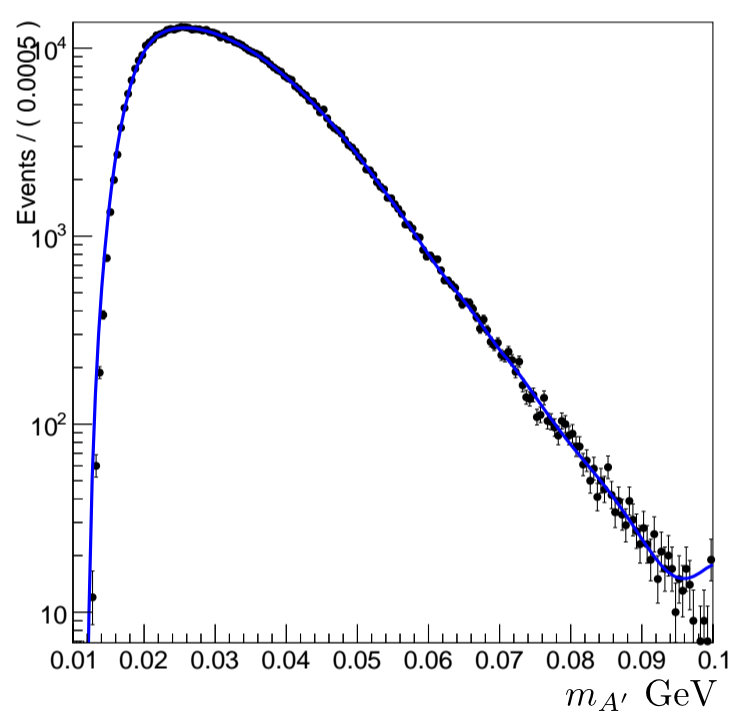
\includegraphics[width=0.7\textwidth]{images/smooth_pdf.png}
%    \caption{Probability density function obtained by applying a smoothing algorithm 
%             to the Heavy Photon Search Monte Carlo invariant mass distribution.}
%    \label{fig:smooth_pdf}
%\end{figure}
 

%Events were sampled from the PDF between 0 and 100 MeV with the total number of
%% What kind of sampling algorithm was used? 
%events, 579336, choosen to match the number observed in data.  The resulting
%pseudo data is binned to match the data distributions with the expectation
%value of each bin Poisson distributed.

\section{Results}

The resulting local $p$-values from a resonance search conducted in the range 
between 20 MeV and 75 MeV are shown on Fig. \ref{}.  The most significant signal
was found at a mass of 28.525 MeV and has a local p-value of $4 \times 10^{-3}$.
After correcting for the LEE, the corresponding global p-value is 
$\sim 10\%$.


\section{Setting Limits}

Since no significant resonances were found, a 90\% confidence upper limit of the number
of signal events at each mass hypothesis was set.  For the purpose of setting
an upper limit, the test statistic define define in equation \ref{}, is inverted.
The resulting statistic used to set an upper limit is then
\begin{equation}
    q_{\mu} = \begin{cases}
        -2 \ln \frac{\mathcal{L}(\mu, \hat{\hat{\theta}})}{\mathcal{L}(0, \hat{\hat{\theta}})} 
            & \hat{\mu} < 0 \\
        -2 \ln \frac{\mathcal{L}(\mu, \hat{\hat{\theta}})}{\mathcal{L}(\hat{\mu}, \hat{\theta})} 
            & 0 <= \hat{\mu} <= 0 \\
             0  & \hat{\mu} > \mu
        \end{cases}
\end{equation}
with the corresponding p-value being given by
\begin{equation}
    p = \int_{q_{\mu,obs}}^{\infty} f(q_{\mu} | \mu) dq_{\mu}.
\end{equation}
In order to find the upper limit, the test above is carried out over a range of
signal yields until a $p$-value of 0.1 (90\% confidence) is found.  The resulting
upper limits are shown on Fig. {}. 

It is often the case that the estimator for the signal yield at a given mass 
is negative.  In this case, it is difficult to interpret whether the experiment
has sensitivity to this region of paramter space.

\section{Setting a limit \epsilon}





